\chapter{Aufgabe 4}


\noindent
In Abbildung~\ref{fig:aussenstelle} ist das gegebene Szenario dargestellt.\\
Aus der geg. Beschreibung geht unmittelbar hervor, dass nur die Benutzer/Systeme der Außenstelle als \textit{Clients} mit den Diensten (\textit{Servern}) der Zentrale kommunizieren sollen.\\

\begin{figure}
    \centering
    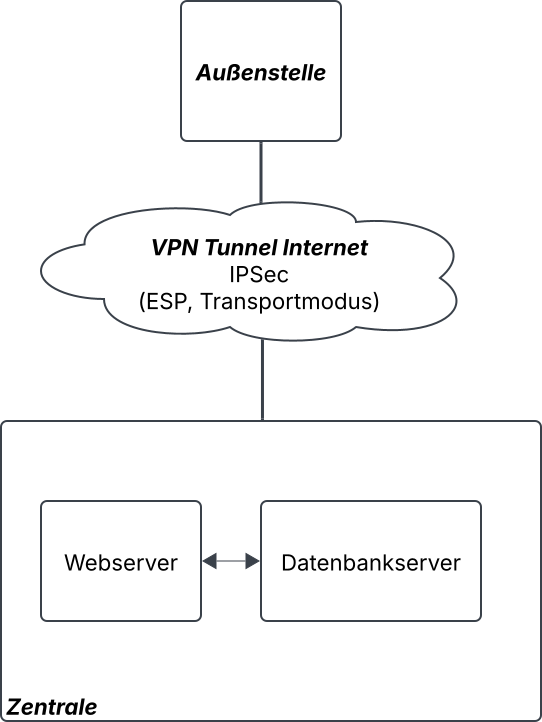
\includegraphics[scale=0.4]{aufgabe 4/img/aussenstelle.svg}
    \caption{Aussenstelle mit VPN-Verbindung in die Zentrale aus dem geg. Szenario (Quelle:eigene)}
    \label{fig:aussenstelle}
\end{figure}

\noindent
Das hierfür genutzte \textit{IPSec} im Transportmodus unter Anwendung von \textit{ESP} (\textit{Encapsulating Security Protocol}) garantiert Vertraulichkeit, da die Daten verschlüsselt werden.\\
Problematisch ist die Tatsache, dass der Original-Header des IP-Pakets nicht gekapselt und demnach auch nicht mitverschlüsselt bzw. zur Erstellung der Authentisierungsdaten verwendet wird - somit ist das Sicherheitsziel \textit{Authentizität} nicht erreicht.\\
Sollte die Architektur beibehalten werden, müsste also eine Kombination aus \textit{ESP} und \textit{AH} (\textit{Authentication Header}) eingesetzt werden - sofern der Transportmodus weiter genutzt werden soll, ansonsten ist die Nutzung von ESP \textit{im Tunnelmodus} ausreichend\footnote{
    siehe hierzu auch Lösungsvorschlag zu Aufgabe 3.
}.

\noindent
Als kostengünstige Alternative würde sich in dem geg. Szenario folgendes anbieten:\\

\noindent
Sicherung der Kommunikation zwischen Client und Server über \textbf{SSL/ TLS} -
da hier eine Kommunikation gesichert werden muss, die nahe an der Anwendungsebene ist (vgl.~\cite[52]{ITS4}).\\
Mit dem Verfahren ist es auch möglich, die Identität in \textit{beider Kommunikationsteilnehmer} zu sichern - also nicht bloß die des Servers (\textit{SSL Record Protocol},~\cite{RFC6101}).\\
Weitere Authentisierungsmaßnahmen der Nutzer gegenüber der Webanwendung sind auf dieser Anwendungsebene zu treffen.\\
Anzumerken ist, dass dies eine \textit{kostengünstige} Lösung ist, aber nicht zwingend die sicherste.
Da aber bei der Auswahl der anzuwendenden Sicherheitsmaßnahmen immer die Verhältnismäßigkeit gewahrt werden soll, und es sich bei den auszutauschenden Daten um ``Veranstaltungshinweise`` und die Buchung von Tickets als gewöhnliche Transaktionen handelt, wie sie im Internet alltäglich geworden sind, kann die Absicherung über SSL/TLS als bewährte Sicherheitsmaßnahme angenommen werden.



